% THE THEME IS WRITTEN AND EDITED BY ABDERAHMANE.KARA 
\usepackage{amsthm}   % For theorems and proof environment
\usepackage{fontspec}
\usepackage{fourier-orns}
% AND IT'S INTENDED PURPOSE IS TO BE SENT FOR MY ANALYSIS
% TEACHER, MR. EL FARISI.
\usepackage{fancyhdr} % DECENT THEME
% \usepackage{fourier-orns} % COOL EMOJIS
\usepackage{hyperref} % refrence links / jumps
\usepackage{etoolbox} %% Provides like a language for advanced customization
\usepackage[a4paper, right = 1in, left = 1in, top = 1in, bottom = 1in]{geometry}
\usepackage{datetime}
\usepackage{lastpage} %% i don't know if i will use it, but possibley
\usepackage{titlesec} %% Modify titles, very imortant for customizing your theme
\usepackage[many]{tcolorbox}
\usepackage{enumerate} % Trivial
\usepackage{cancel} % Trivial
\usepackage{tikzsymbols} % Tikz symbols
\usepackage[dvipsnames]{xcolor} % provides extra color with that option
\usepackage{import} % import images
\usepackage{amsmath,amssymb} % math tools, and cool font
\usepackage{unicode-math}

\setmainfont{palatino}
\setmathfont{Asana Math}

	% DEFAULT LATEX THAT I ALWAYS USE
% \setmainfont{palatino}    
% \setmathfont{Asana Math}

\usepackage{tikz}  % tikz picture 
\usepackage{bookmark} % useful for rendering, i don't know exactly why
\usepackage{graphicx} % self descriptive

% \usepackage{mathpazo} % i forgot :)

\usepackage{fontawesome5} % amazing emojis and other stuf

% \usepackage{courier}
% \usepackage{helvet}
% \usepackage{lmodern}

\linespread{1.5}

\pagestyle{fancy}

\fancyhead[R]{\leftmark}
\fancyhead[L]{}

\usepackage{shadowtext}



% \titleformat{\chapter}[block]
%   {\bf\fontfamily{ppl}\selectfont\Large}
%   {CHAPTER : \Huge\textbf{\shadowtext{ \thechapter}}}
%   {1cm}
%   {\MakeUppercase}
% 
\newfontface\frakturfont{TeX Gyre Schola}[Contextuals={WordInitial,WordFinal}]

\titleformat{\chapter}[block]
{

\begin{tikzpicture}%[overlay]
	\draw[double,line width = 0.5mm, double distance = 0.5mm] (0,0) rectangle (\textwidth,2);
	\node[anchor=west]  at (\textwidth/24,1) {\huge \it CHAPTER };
		\node[anchor=east]  at (\textwidth * 23/24, 1) {
			\Huge \it \thechapter };
\end{tikzpicture}
}
{
	\begin{tikzpicture}[overlay]
	\end{tikzpicture}
}
{0cm}
{\huge}
 

 \titleformat{\section}[block]
 {
	 \Large \bf
 }
 {\Large  \thesection.}
 {0.5cm}
 {}
% 
% 
 \newcommand{\divider}
 {
 	\begin{center}
 	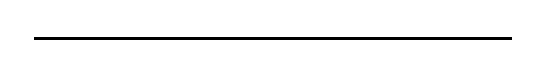
\begin{tikzpicture}
 		\draw[thick, black] (0.25*\textwidth, 0) -- (0.75*\textwidth, 0);
 		\node[rotate = 360 - 90, xshift = -0.6pt, yshift = 1pt] at (0.25*\textwidth,0){\decotwo};
 		\node[rotate = 90, xshift = -0.6pt, yshift = 1pt] at (0.75*\textwidth,0){\decotwo};
 	\end{tikzpicture}
 	\end{center}
 }
 
\newcommand{\signature}
{
	\begin{tikzpicture}[remember picture,overlay]
	\node[fill = YellowOrange!20!white] 
	at ([yshift = 1cm, xshift = -3cm]current page.south east) 
	{\fontsize{10pt}{0pt}{\itshape Kara.$\mathcal{A}$}};
	\end{tikzpicture}
}



\newtcolorbox[auto counter, number within= section]{definition}[1][]
 {
	 title = Definition~\thetcbcounter~ #1,
 	enhanced,
 	boxrule = 1pt,
 	fonttitle = \bf \color{black},
 	colback = white,
 	breakable,
        sharp corners,
 	% frame hidden,
        borderline west = {2pt}{0pt}{black},
	detach title,
	before upper = \tcbtitle \\,
	% attach title to upper = 
	% {
	% 	\\ \tld
	% },
	% after title = {\\},
	% before upper = \quad,
 	% attach boxed title to top left =
 	% {
 	% 	xshift = 0cm,
 	% },
 	% boxed title style =
 	% {
 	% 	colback = white,
 	% 	frame hidden
	% },
 }
 \newcommand{\lecday}[1][]
{
    \def\datee{#1}
    \fancyhead[L]{\datee}
}

\newtcolorbox[auto counter,number within= section]{theorem}[1][]
 {
	title = Theorem~\thetcbcounter~ #1,
 	enhanced,
 	boxrule = 1pt,
 	fonttitle = \bf \color{black},
 	colback = white,
 	breakable,
        sharp corners,
 	frame hidden,
        borderline west = {2pt}{0pt}{black},
	detach title,
	before upper = \tcbtitle \\,
 }

 \newtcolorbox[auto counter, number within = section]{proposition}[1][]
 {
	title = Proposition~\thetcbcounter #1,
 	enhanced,
 	boxrule = 1pt,
 	fonttitle = \bf \color{black},
	colback = white,
 	breakable,
        sharp corners,
 	frame hidden,
	detach title,
	before upper = \it \tcbtitle \quad ,
 }
 \newtcolorbox[auto counter, number within = section]{corollary}[1][]
 {
	title = Corollary~\thetcbcounter #1,
 	enhanced,
 	boxrule = 1pt,
 	fonttitle = \bf \color{black},
	colback = white,
 	breakable,
        sharp corners,
 	frame hidden,
	detach title,
	before upper = \it \tcbtitle \quad ,
 }
 \newtcolorbox{example}[1][]
 {
	title = Example, 
 	enhanced,
 	boxrule = 1pt,
 	fonttitle = \bf \color{black},
	colback = white,
 	breakable,
        sharp corners,
	detach title,
	before upper = \it \tcbtitle \quad ,
 }

 \newtcolorbox{remark}[1][]
 {
	title = Remark, 
 	enhanced,
 	boxrule = 1pt,
 	fonttitle = \bf \color{black},
	colback = white,
 	breakable,
        sharp corners,
	detach title,
	before upper =  \tcbtitle \it \quad ,
 }


% \newtcolorbox{proof}
% {
%      title = proof ,
% 	enhanced,
% 	boxrule = 1pt,
% 	fonttitle = \it \color{black},
%      colback = white,
% 	breakable,
%        sharp corners,
%      detach title,
%      before upper = \it \thetcbtitle \\ ,
% }





 \newcommand{\integral}[4]{\int\limits_{#1}^{#2} #4 d#3}
\newcommand{\limit}[3]{\lim\limits_{#1 \rightarrow #2} #3}
\newcommand{\strone}[2]{\left[ \begin{gathered}#1\\ #2\end{gathered} \right] }
\newcommand{\strtwo}[2]{\left\{ \begin{gathered}#1\\ #2\end{gathered} \right\} }
\newcommand{\strthree}[2]{\left\lfloor \begin{gathered}#1\\ #2\end{gathered} \right\rfloor }


\newcommand{\startbf}[1]{\text{\bfseries{#1}}}
\newcommand{\sett}[1]{\left\{ #1 \right\}}
\newcommand{\thesis}[1]{\left( #1 \right)}
\newcommand{\brkt}[1]{\left[ #1 \right]}
\newcommand{\floor}[1]{\left\lfloor #1 \right\rfloor}


\DeclareMathOperator{\img}{im} % Image
\DeclareMathOperator{\Img}{Im} % Image
\DeclareMathOperator{\coker}{coker} % Cokernel
\DeclareMathOperator{\Coker}{Coker} % Cokernel
\DeclareMathOperator{\Ker}{Ker} % Kernel
\DeclareMathOperator{\rank}{rank}
\DeclareMathOperator{\Spec}{Spec} % spectrum
\DeclareMathOperator{\Tr}{Tr} % trace
\DeclareMathOperator{\pr}{pr} % projection
\DeclareMathOperator{\ext}{ext} % extension
\DeclareMathOperator{\pred}{pred} % predecessor
\DeclareMathOperator{\dom}{dom} % domain
\DeclareMathOperator{\ran}{ran} % range
\DeclareMathOperator{\Hom}{Hom} % homomorphism
\DeclareMathOperator{\Mor}{Mor} % morphisms
\DeclareMathOperator{\End}{End} % endomorphism


\newcommand{\lm}{\ensuremath{\lambda}}
\newcommand{\eps}{\ensuremath{\epsilon}}
\newcommand{\veps}{\ensuremath{\varepsilon}}
\newcommand{\al}{\ensuremath{\alpha}}
\newcommand{\bb}{\ensuremath{\beta}}
\newcommand{\cc}{\ensuremath{\gamma}}
\newcommand{\dd}{\ensuremath{\delta}}
\newcommand{\DD}{\ensuremath{\Delta}}
\newcommand{\ff}{\ensuremath{\phi}}
\newcommand{\FF}{\ensuremath{\varphi}}

\newcommand{\RR}{\mathbb{R}}
\newcommand{\RO}{\mathcal{R}}
\newcommand{\EE}{\mathbb{E}}
\newcommand{\CC}{\mathbb{C}}
\newcommand{\RW}{\mathbb{R}^2}
\newcommand{\RT}{\mathbb{R}^3}
\newcommand{\RN}{\mathbb{R}^n}
\newcommand{\DS}{\mathcal{D}}

\newcommand{\KK}{\mathbb{K}}
\newcommand{\KW}{\mathbb{K}^2}
\newcommand{\KT}{\mathbb{K}^3}
\newcommand{\KN}{\mathbb{K}^n}

\newcommand{\NN}{\mathbb{N}}

\newcommand{\PS}{\mathcal{P}}
\newcommand{\AS}{\mathcal{E}}
\newcommand{\FS}{\mathcal{F}}
\newcommand{\LS}{\mathcal{L}}
\newcommand{\MS}{\mathcal{M}}
























